\section{Related Work}


\begin{figure*}
    \centering
    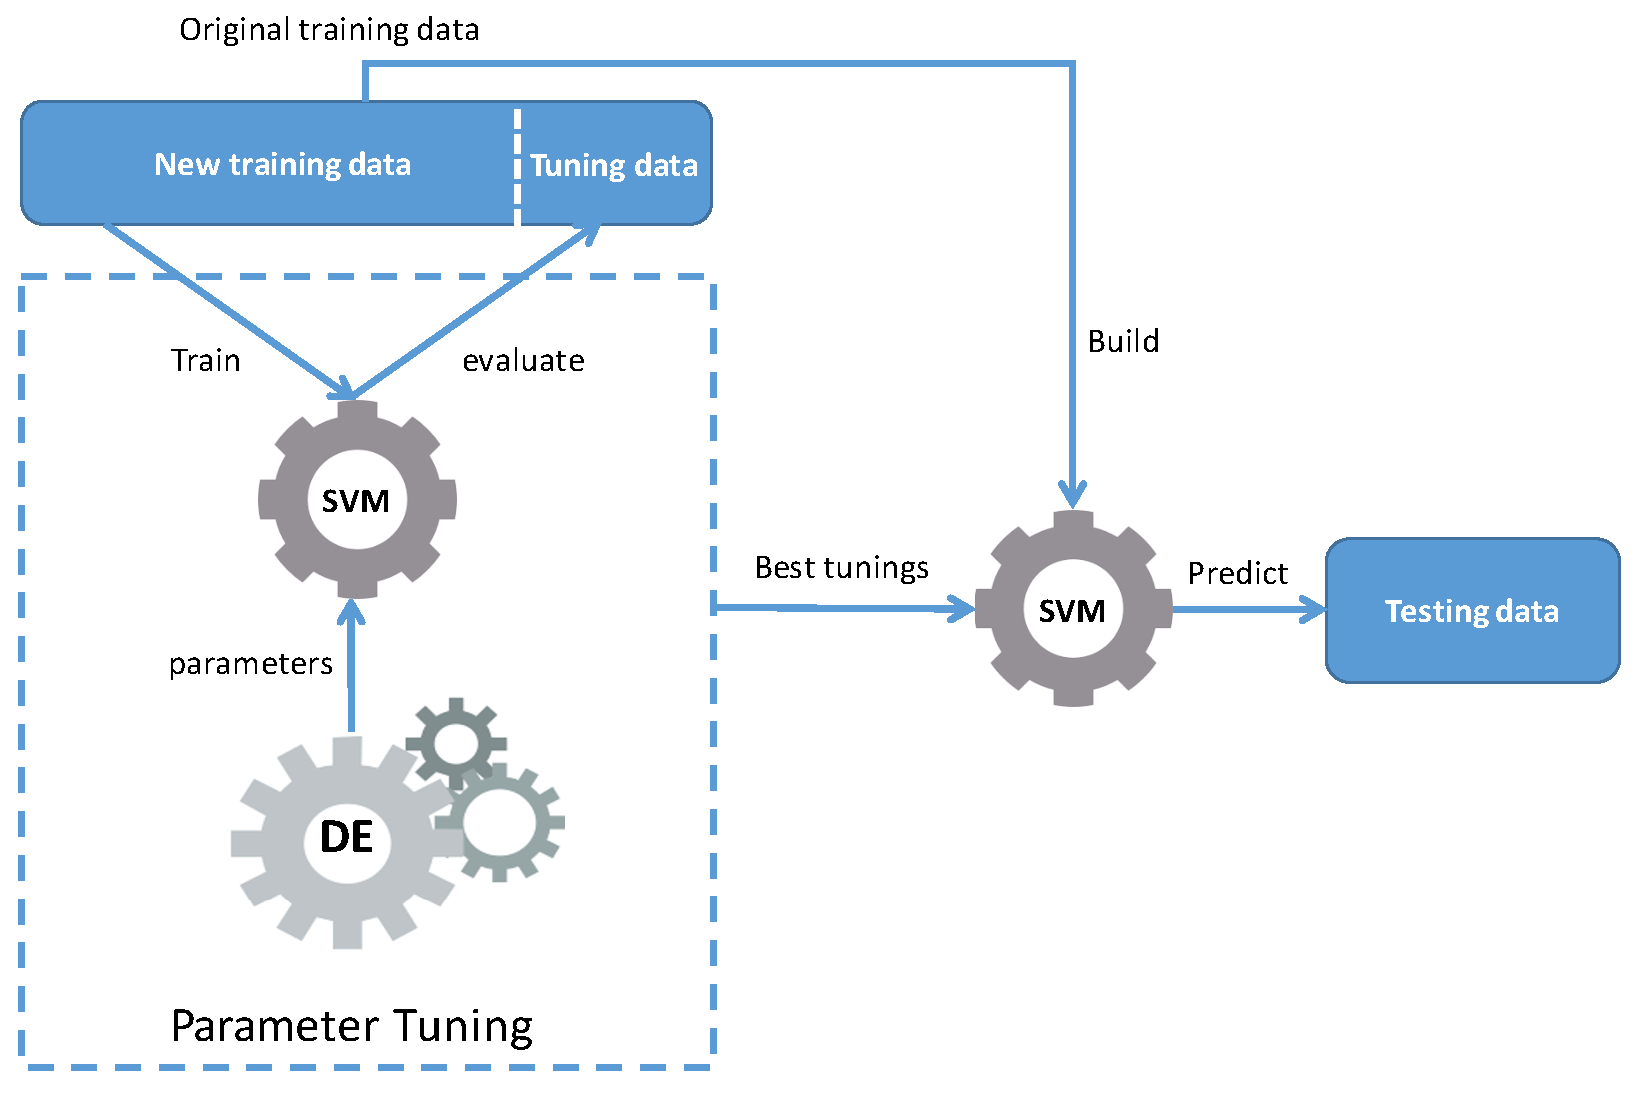
\includegraphics[width=6.45in]{pic/workflow.pdf}
    \caption{Caption}
    \label{fig:my_label}
\end{figure*}


\subsection{Deep Learning in SE}
With the vast amounts of computational power and data, 
deep learning has been proven to be a very powerful method 
by researchers in many fields\cite{lecun2015deep}, like computer vision and natural language processing\cite{krizhevsky2012imagenet,mikolov2013distributed,sutskever2014sequence}. 
Recently, it also has attracted  attentions from researchers and practitioners in software
 community\cite{wang2016automatically, gu2016deep, xu2016predicting,white2016deep,white2015toward,lam2015combining,choetkiertikul2016deep}.
 These researchers applied  deep learning techniques to solve various problems,
 including defect prediction, bug localization, clone code detection, API recommendation, 
 effort estimation and linkable knowledge prediction.
 
By carefully reading, these work can be divided into the following two categories:
 
\begin{itemize}
\item treat deep learning as a feature extractor, and then apply other regular machine learning to do further job.
\item apply deep learning directly to solve the problems.
\end{itemize}

Lam et al.~\cite{lam2015combining}  proposed an approach to apply deep neural network
 in combination with rVSM to automatically locate the potential buggy files for a given
 bug report. By comparing it to the baseline methods(learn-to-rank\cite{ye2014learning}, 
 BugLocator~\cite{zhou2012should}), authors reported $8-20.8\%$  and $2.7-20.7\%$ 
 higher top-1 accuracy than baseline methods, respectively. The training time for deep neural
 network was reported from 70 to 122 minutes on a computer with 32 cores CPU,
 126 GB RAM machine. However,
 no such time information reported about baseline methods.
 
 Wang et al.~\cite{wang2016automatically} applied deep belief network to automatically
 learn semantic features from token vectors extracted from the studied program. After
 that, Naive Bayes and Logistic Regression methods are used to evaluate the effectiveness
 of such feature generation method as well as PROMISE and AST features. In terms of
 running time, Wang et al. only reported time for generating semantics features with deep belief network, which
 ranged from 8 seconds to 32 seconds. However, the time for training and tuning deep belief network is
 missing. Furthermore, to evaluate the effectiveness of deep belief network in terms of time cost, 
 it would be favorable to include all the time spent on feature extraction, including
 paring source code, token generation.
 
 Choetkiertikul et al.~\cite{choetkiertikul2016deep} proposed to apply deep learning techniques
 to solve effort estimation problem, where they used long short-term memory(LSTM) to learn
 feature vectors from the title, description and comments associated with an issue report and
 regular machine learning techniques applied afterwards. LSTM was reported to have a 
 significant improvement over the baseline method bag-of-word. No further information regarding
 runtime was reported for both methods.
 
 White et al.~\cite{white2015toward, white2016deep} applied
 recurrent neural networks, one type of  deep learning techniques, 
 to address code clone detection and code suggestion. As they reported,
 the average training time for 8 projects were ranging from 34 seconds
  to 2977 seconds for each epoch on a two 3.3 GHz
 CPUs computer and each project required at least 30 epochs~\cite{white2016deep}.
 For the {\it JDK} project in their experiment, it would take 25 hours 
 on the same computer to train the models before getting prediction.
 For the time cost for code suggestions, authors didn't mention any related information~\cite{white2015toward}.

Gu et al.~\cite{gu2016deep} proposed  a recurrent neural network(RNN)
 based method, D{\scriptsize EEP}API, to generate API usage sequences for a given natural language query. 
 Compared with the baseline method {\it SWIM}~\cite{raghothaman2016swim} and 
 {\it Lucene + UP-Miner}~\cite{wang2013mining},  D{\scriptsize EEP}API has improved the performance a lot.
 However, one can't ignore the fact that such model was trained with a Nivdia K20 GPU for about 240 hours.
 
 Xu et al.~\cite{xu2016predicting} utilized neural language model and  
 convolutional neural network(CNN) to  learn word-level and document-level features to
 predict semantically linkable knowledge units in Stack Overflow. 
 In terms of performance metrics, like precision, recall and F1-score,
 CNN method was evaluated much better than 
 the baseline method support vector machine(SVM). 
 However, the time cost for training CNN is not ignorable as it took
 14 hours to train CNN model on a 2.5GHz PC with 16 GB RAM 
 to achieve the relative low loss convergence.
 
 In summary, all the above work authors are trying hard to promote deep learning in software
 engineering community. They presented somewhat or even much better results compared with
 the baseline methods. However, they either didn't present the computational and time cost, like \cite{white2016deep,white2015toward,lam2015combining,choetkiertikul2016deep}, or simply listed
 the cost as it is without further discussion\cite{wang2016automatically, gu2016deep, xu2016predicting}. Without comparing cost with the baseline methods like all above paper,
 we actually don't have a concrete idea about how well deep learning can solve software engineering problems in terms of both benefits and costs. Especially when we don't have much knowledge about
 whether such problems are suitable for deep learning. 
 
As deep learning techniques cost huge amount of time and computational
resources to train its model,
one might ask question whether the improvements from deep learning is worth
the costs. {\it Are there any simple techniques that achieve similar improvements
with less resource costs?} and {\it what might be the baseline methods to compare with
when deep learning is applied?}

In this paper, we revisit the research problems 
from Xu et al.\cite{xu2016predicting} work, and by applying parameter tuning 
to SVM algorithms, we find that the results we've got, on average, are even 
better than their CNN results with quite less training and tuning time.
Specifically, SVM with optimal tunings have won over deep learning 
in $\frac{8}{12}$ performance scores and for those $\frac{4}{12}$,
tuned SVM  does not lose much. However, CNN took 14 hours to achieve
those scores and parameter tuning only require 10 minutes, which is almost 80X faster.




\subsection{Parameter Tuning in SE}
Machine learning algorithms are designed to explore the instances
to learn the bias. However, most of these algorithms are controlled by parameters
, like the depth of the tree in CART, which would change the
exploration behavior if set different tunings. This parameter(or Hyper-parameter)
tuning problem is well explored in other community \cite{bergstra2012random,li2016hyperband}.
In software engineering community, this issue is ignored for quite
long time and recently, there's been a trend to starting investigation on such effect.

Fu et al.\cite{fu2016tuning} surveyed hundreds of highly 
cited software engineering paper in area of defect prediction. 
Their observation is that most software engineering  researchers
didn't acknowledged the impact of tunings 
(exceptions: \cite{lessmann2008benchmarking,tantithamthavorn2016automated}) and
use the ``off-the-shelf''data miners. For example, 
Elish et al.\cite{elish2008predicting} compared support vector machines
to other data miners for the purposes of defect prediction.
However, the Elish et al. paper makes no mention of any SVM tuning study.
For those two exceptions\cite{lessmann2008benchmarking,tantithamthavorn2016automated}, 
they simply apply grid search to explore the potential parameter space for optimial tunings.
However, Bergstra et al.\cite{bergstra2012random} and 
Fu et al.\cite{fu2016differential} argue that random search and 
differential evolution(DE) algorithm are better than 
grid search in terms of efficiency and performance.
Fu et al showed that finding useful tunings for software defection is remarkably easy and fast using DE.

Recently, Argrawa et al.\cite{agrawal2016wrong} investigated 
impact of parameter tuning on Latent Dirichlet Allocation(LDA),
which is a widely used technique in software engineering field
to find related topics within unstructured text, 
like topics analytics in stack overflow \cite{barua2014developers}
and source code analysis \cite{binkley2014understanding}.
According to Argrawa et al., LDA suffers from the instability issue.
Parameters within LDA are one reason to cause such problem. However,
quite few researchers(4 out of 57 papers) using LDA worried about
that tuning might have a large impact on the results. By applying DE to find 
optimal tunings,  Argrawa et al. find that the resultant LDA is able to generate more stable results
for both supervised learning and unsupervised learning.
They also confirm the statement made by Fu et al.\cite{fu2016tuning} that
parameter tuning with DE is not extremely slow and DE is easy to implement.

In this work, parameter tuning is applied to the baseline method for Deep Learning
to better understand how deep learning perform in terms of efficiency and performance.
Since (a)tuning with DE is easy to implement and fast to run; (b) it's shown to be able
to improve learners' performance, it will not introduce much overhead to the baseline method.

To our best knowledge, this is the first paper
applying parameter tuning to the baseline method for Deep learning methods in 
software engineering community. Our results show that no further software analytics
paper with Deep Learning just use ``off-the-shelf'' data miners as the baseline
method to compare with. Furthermore, since Deep Learning is such a resource consuming
technique and software analytics tasks are not extremely complicated, the cost for 
both baseline methods and Deep learning method should be supplied.











